%!TEX root = skripsi.tex
%-----------------------------------------------------------------------------%
\chapter{\babTiga}
%-----------------------------------------------------------------------------%
%-----------------------------------------------------------------------------%
\section{Rancangan Sistem}
%-----------------------------------------------------------------------------%
% Ide, model matematik, rumus, fitur, jangan m=ngomongin teknologi (java, keras, dll), word2vec boleh %
Sistem yang akan \saya~buat dalam penelitian ini sesuai dengan rancangan arsitektur sistem pada gambar \ref{fig:arsitektur_sistem}.
\begin{figure}
  \centering
  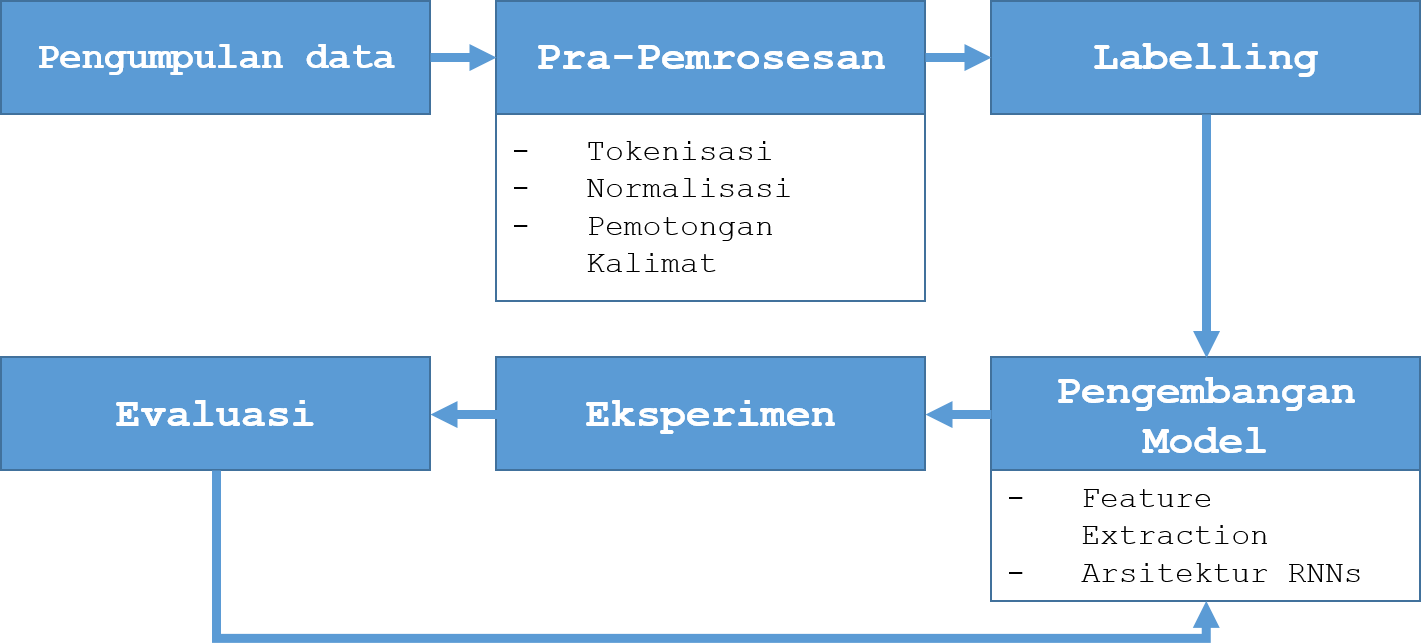
\includegraphics[width=\linewidth]{images/arsitektur}
  \caption{Rancangan Arsitektur Sistem}
  \label{fig:arsitektur_sistem}
\end{figure}

Berikut merupakan penjelasan alur dalam rancangan arsitektur sistem.
	\subsection{Pengumpulan Data}
	Pengumpulan data dilakukan dengan tujuan untuk mendapatkan data \textit{training} dan \textit{testing} sebagai \textit{input} sistem \mer~yang diusulkan. Data yang dimaksud merupakan teks dari forum kesehatan \textit{online} dari berbagai sumber. 
	
	\subsection{Pra-Pemrosesan}
	Pra-pemrosesan dilakukan dengan tujuan supaya teks yang diberikan mampu dibaca oleh sistem \mer. Dalam tahap ini, ada dua pekerjaan utama yang perlu dilakukan, yaitu:
	\begin{enumerate}
		\item Pembersihan data\\
		Langkah ini dilakukan dengan tujuan untuk membersihkan dokumen dari berbagai karakter yang tidak terdapat dalam karakter ASCII. Selain itu, perlu juga pengubahan beberapa tanda baca/token menjadi 1 token tersendiri. Misalnya sebuah token tautan (\textit{www.alodokter.com/asma/pengobatan}) diganti menjadi token "url".
		\item Tokenisasi\\
		Tokenisasi dilakukan untuk mendapatkan token yang paling tepat sebagai satu buah kata. Hal ini perlu dilakukan untuk menghindari beberapa kelompok token berbeda yang tergabung. Misalnya karakter abjad dengan karakter angka atau karakter abjad dengan karakter tanda baca dipisahkan berdasarkan kelompoknya.
		\item Pemotongan kalimat\\
		Untuk menghindari jumlah token yang timpang dalam kalimat yang berbeda dan data yang \textit{sparse}, diperlukan pemotongan kata yang tepat. Langkah-langkah yang diperlukan untuk melakukan pemotongan kata yaitu:
		\begin{enumerate}
			\item memisahkan kalimat berdasarkan tanda baca (.!?,),
			\item apabila suatu kalimat memiliki jumlah kata yang sedikit (misal diberikan batasan minimal 10 kata dalam satu kalimat), kalimat tersebut digabungkan dengan kalimat setelahnya.
		\end{enumerate}
	\end{enumerate}
	
	\subsection{Pelabelan}
	Pada tahap ini, \saya~melakukan pelabelan pada dokumen teks yang merupakan hasil pada tahap sebelumnya dengan label \disease, \symptom, \drug~dan \treatment. Berikut merupakan penjelasan dari masing-masing label:
	\begin{enumerate}
		\item \Disease\\
		Entitas \disease~yang dimaksud pada penelitian ini yaitu nama dari suatu penyakit. Penyakit merupakan keadaan abnormal yang timbul pada tubuh manusia. Contoh dari entitas \disease~yaitu:
		\begin{description}
			\item[$\bullet$] Skizofrenia
			\item[$\bullet$] Trikotilomania
			\item[$\bullet$] Diabetes melitus
		\end{description}
	
		\item \Symptom\\
		Entitas \symptom~yang dimaksud pada penelitian ini yaitu fenomena yang dialami oleh seseorang yang terkena suatu penyakit. Contoh dari entitas \symptom~yaitu:
		\begin{description}
			\item[$\bullet$] Napas berbunyi
			\item[$\bullet$] Benjolan di daerah perut
			\item[$\bullet$] Nyeri saat BAK
		\end{description}
	
		\item \Drug\\
		Entitas \drug~merupakan entitas nama obat dari suatu penyakit yang memiliki fungsi untuk mengurangi atau menyembuhkan penyakit tersebut. Contoh dari entitas \drug~yaitu:
		\begin{description}
			\item[$\bullet$] Paracetamol
			\item[$\bullet$] Diltiazem
			\item[$\bullet$] eritropoetin-alfa
		\end{description}
	
		\item \Treatment\\
		Entitas \treatment~merupakan cara atau langkah penyembuhan dari suatu penyakit. Contoh dari entitas \treatment~yaitu:
		\begin{description}
			\item[$\bullet$] Pemeriksaan darah rutin
			\item[$\bullet$] Penilaian denyut kapiler
			\item[$\bullet$] Terapi inhalasi
		\end{description}
	\end{enumerate}
		
	\subsection{Pengembangan Model}
	Pada tahap ini, \saya~melakukan pengusulan dan perancangan model yang nantinya akan \saya~evaluasi pada tahap eksperimen. Dalam mengembangkan model, terdapat dua pekerjaan yang\saya~lakukan, yaitu:
	
	\subsubsection{Ekstrasi Fitur}
	Pada tahap ini, \saya~melakukan ekstraksi fitur dari dokumen yang telah diberi label entitas. Ada beberapa fitur yang \saya~usulkan dalam penelitian ini yang nantinya \saya~kombinasikan supaya mendapatkan hasil terbaik. Fitur-fitur tersebut yaitu:
	\begin{enumerate}
		\item Fitur 1: Kata itu sendiri\\
		Fitur ini merupakan fitur kata dalam representasi vektor. Untuk mendapatkan representasi vektor dari masing-masing kata, penulis menggunakan \textit{word embedding}. Terdapat beberapa langkah yang perlu \saya~lakukan dalam memanfaatkan \textit{word embedding} ini, yaitu:
		\begin{enumerate}
			\item Pengumpulan data \textit{training} untuk \textit{word embedding}
			\item \textit{Training} untuk mendapatkan model \textit{word embedding}
			\item Pengubahan kata menjadi vektor dari model yang didapatkan
		\end{enumerate}
		
		\item Fitur 2: \textit{Part of Speech Tag} (POS-Tag)\\
		Fitur ini merupakan fitur \textit{tag} yang dimiliki setiap kata yang diusulkan oleh \cite{abacha2011medical} dalam penelitiannya di bidang \mer. Model yang digunakan merupakan model POS-Tag berbahasa Indonesia.
		
		\item Fitur 3: \textit{Stopword}\\
		Fitur ini merupakan fitur yang berisi vektor suatu kata merupakan \textit{stopword} atau bukan.
		
		\item Fitur 4: Kamus kesehatan\\
		Fitur kamus kata merupakan fitur yang berisi informasi suatu kata terdapat di dalam kamus kesehatan atau tidak. Pada penelitian ini, kamus kesehatan yang dipakai ada sejumlah entitas yang akan dikenali, yaitu kamus \disease, kamus \symptom, kamus \drug~dan kamus \treatment.\
		
		\item Fitur 5: Frasa kata benda\\
		Menurut \cite{hs2005bahasa}, frasa kata benda sendiri merupakan kelompok kata benda yang dibentuk dengan memperluas kata benda ke sekelilingnya. Fitur frasa kata benda yang \saya~gunakan dalam penelitian merupakan fitur yang berisi informasi suatu kata atau kumpulan kata merupakan frasa kata benda atau bukan. Dalam menentukan suatu kata merupakan frasa atau bukan, penulis menggunakan aturan pembentukan frasa yang digunakan pada bahasa Indonesia, yaitu:
		\begin{description}
		 	\item[$\bullet$] NP : NN
		 	\item[$\bullet$] NP : NNP
		 	\item[$\bullet$] NP : PR
		 	\item[$\bullet$] NP : PRP
		 	\item[$\bullet$] NP : NN + NN
		 	\item[$\bullet$] NP : NN + NNP
		 	\item[$\bullet$] NP : NN + PR
		 	\item[$\bullet$] NP : NN + PRP
		 	\item[$\bullet$] NP : NN + JJ
		 	\item[$\bullet$] NP : DT + NN
		 	\item[$\bullet$] NP : RB + NN
		 	\item[$\bullet$] NP : CD + NN
		 	\item[$\bullet$] NP : NND + NN
		 \end{description}
	 
		 \item Fitur 6: Frasa verbal\\
		 Fitur frasa kata kerja merupakan fi
	\end{enumerate}
	
	\subsection{Eksperimen}
	Dalam melakukan Eksperimen, \saya~menggunakan \textit{Recurrent Neural Network}. \textit{Tools} yang \saya~gunakan yaitu Keras. Keras merupakan \textit{library} untuk \textit{Deep Learning} yang \textit{high level} yang ditulis dalam bahasa pemrograman python. Keras yang \saya~gunakan berjalan di atas Theano.
	Sebelum memulai eksperimen, \saya~membagi data menjadi beberapa bagian untuk melakukan \textit{n-fold cross validation}. Hal ini \saya~lakukan karena data yang digunakan sedikit. Dalam melakukan pembagian data, \saya~menggunakan program buatan \saya~sendiri dengan menggunakan bahasa pemrograman Python.
	Setelah data telah terbagi menjadi n-bagian, \saya~melakukan pengkombinasian fitur-fitur supaya mendapatkan hasil terbaik.
%-----------------------------------------------------------------------------%
\section{Data}
%-----------------------------------------------------------------------------%
Penelitian ini memerlukan data berupa berkas audio bacaan seluruh ayat \quran~di juz 30 dari berbagai qari. Karena sistem yang dikembangkan adalah pengenalan suara per ayat, maka data yang diperlukan berupa bacaan \quran~yang sudah dipotong per ayat. Dengan kata lain, satu \f{instance} data merepresentasikan satu ayat \quran~yang dibaca oleh seorang qari. Berikut adalah langkah-langkah untuk memperoleh data tersebut dan memilih data yang tepat untuk digunakan dalam eksperimen.

  \subsection{Pengambilan Data} \label{pengambilan data}
  Data diperoleh dengan cara mengunduh dari beberapa sumber, yaitu \url{http://everyayah.com}, \url{http://tanzil.net}, dan \url{http://recitequran.com}. Tiga sumber tersebut memberi penomoran yang urut pada datanya. Penomoran berkas yang urut memudahkan proses pengunduhan untuk dilakukan secara otomatis menggunakan bantuan program. Nama berkas untuk surat ke-\f{s} dan ayat ke-\f{a} adalah \f{sssaaa.mp3}. Contoh untuk surat ke-78 ayat pertama adalah \f{078001.mp3} dan surat ke-114 ayat ke-6 adalah \f{114006.mp3}. Data yang diambil adalah seluruh surat, mulai dari surat ke-78 sampai dengan surat ke-114 (seluruh surat dalam \quran~di juz 30). Total ayat dari surat-surat yang diambil adalah 564 ayat untuk masing-masing qari.

  Di dalam tiga \f{website} yang telah disebutkan sebelumnya tersedia data berupa berkas mp3, di mana satu berkas merepresentasikan satu ayat. Masing-masing berkas memiliki informasi detil yang berbeda-beda, terutama pada \f{duration}, \br, dan \f{channel}. Tabel \ref{table:format berkas 078007 alafasy} menyajikan informasi detil salah satu berkas, yaitu surat An-Naba' ayat 7 dengan qari Mishary Rashid Alafasy.

  \begin{table}
    \centering
    \caption{Informasi Detil Surat An-Naba' Ayat 7 dengan Qari Mishary Rashid Alafasy}
    \begin{tabular}{|c|c|}
      \hline
      Format                         & MPEG Audio \\ \hline
      Format version                 & Version 1 \\ \hline
      Format profile                 & Layer 3 \\ \hline
      Mode                           & Joint stereo \\ \hline
      Mode extension                 & MS Stereo \\ \hline
      Duration                       & 3.866 s \\ \hline
      Bit rate mode                  & Constant \\ \hline
      Bit rate                       & 128 Kbps \\ \hline
      Channel(s)                     & 2 channels \\ \hline
      Sampling rate                  & 44.1 KHz \\ \hline
      Compression mode               & Lossy \\ \hline
      Stream size                    & 60.4 KiB (99\%) \\ \hline
      Writing library                & LAME3.96r \\ \hline
      Encoding settings              & -m j -V 4 -q 3 -lowpass 17.5 -b 128 \\ \hline
    \end{tabular}
    \label{table:format berkas 078007 alafasy}
  \end{table}



  \subsection{Pembuangan Data Duplikat}
  Dari tiga sumber yang telah disebutkan pada Bab \ref{pengambilan data}, diperoleh data bacaan \quran~lebih dari 50 qari berbeda. Namun di antara data-data tersebut, ada beberapa data yang duplikat, yaitu data dengan nama berkas berbeda tetapi sebenarnya memiliki suara yang sama persis. Hal ini dikarenakan ada sedikit perbedaan dari masing-masing sumber data dalam menamai qari. Misalnya dalam \url{http://everyayah.com} terdapat qari dengan nama ``Alafasy\_128kbps'' dan dalam \url{http://tanzil.net} terdapat qari dengan nama ``afasy''. Dua nama tersebut merujuk ke orang yang sama. Untuk mengetahui bahwa dua berkas memiliki konten audio yang sama tidak dilihat dari nama berkasnya, tetapi menggunakan teknik lain. Dalam penelitian ini teknik yang digunakan adalah perbandingan nilai MFCC. Langkah-langkah dari teknik tersebut adalah sebagai berikut.

  \begin{enumerate}
    \item \label{step:pilih ayat} \textbf{Menentukan satu ayat yang akan menjadi acuan}\\
    Ayat yang dipilih boleh yang mana saja, tetapi disarankan bukan ayat pertama dari setiap surat. Ayat pertama dari setiap surat terkadang mengandung bacaan \f{basmalah}\footnote{sebutan untuk bacaan ``\<بِسْمِ اللَّـهِ الرَّحْمَـٰنِ الرَّحِيمِ>''.} yang sebenarnya bukan merupakan bagian dari ayat tersebut, karena bacaan tersebut sifatnya opsional untuk dibaca di awal surat. Ayat yang digunakan pada langkah selanjutnya hanya ayat yang terpilih pada langkah ini. Dalam penelitian ini ayat yang digunakan sebagai acuan adalah ayat ke-6 dari surat ke-114.
    
  	\item \label{step:hitung mfcc} \textbf{Ekstraksi MFCC dari semua qari}\\
  	Dengan mengacu pada ayat yang ditentukan di langkah \ref{step:pilih ayat}, audio bacaan \quran~masing-masing qari diekstrak nilai MFCC-nya. Dalam penelitian ini, parameter koefisien MFCC yang digunakan adalah 13. Hasil dari ekstraksi nilai MFCC berupa matriks berukuran $13\times K$, di mana $K$ merepresentasikan banyaknya \fr. Nilai $K$ bervariasi, bergantung pada durasi audio yang diekstrak. Kemudian, nilai rata-rata dari matriks $13\times K$ pada setiap barisnya dihitung, sehingga terbentuk vektor kolom dengan panjang 13. Vektor kolom adalah matriks yang memiliki tepat 1 kolom. Penghitungan rata-rata dilakukan per baris supaya panjang vektor dari hasil perhitungan ini konstan, yaitu 13. Karena jika yang dihitung nilai rata-rata per \fr, maka hasilnya tentu bervariasi sesuai dengan banyak \fr~dari masing-masing nilai MFCC, yang dipengaruhi oleh durasi audio. Panjang setiap vektor dari langkah ini haruslah sama supaya masing-masing vektor dapat dihitung nilai jaraknya.
  	
  	\item \label{step:hitung jarak} \textbf{Menghitung jarak dari setiap pasang data}\\
    Setiap pasang vektor yang terbentuk dari langkah \ref{step:hitung mfcc} kemudian dihitung nilai jaraknya. Sehingga akan terbentuk matriks D berukuran $N\times N$ yang berisi nilai-nilai jarak tersebut, di mana $N$ adalah banyaknya qari. Baris ke-i dan kolom ke-j menyatakan nilai jarak dari qari ke-i dengan qari ke-j. Penelitian ini menggunakan nilai jarak \f{euclidean distance}\footnote{persamaan \ref{equ:euclideandistance}}.
  	
  	\item \label{step:clustering} \textbf{Mengelompokkan matriks D}\\
    Kumpulan sel di matriks D hasil dari langkah \ref{step:hitung jarak} kemudian dikelompokkan ke dalam 4 kelompok menggunakan teknik \f{k-means clustering}. Pembagian ke dalam 4 kelompok ini dimaksudkan supaya data terbagi ke dalam kelompok \f{mirip}, \f{sedikit mirip}, \f{tidak terlalu mirip}, dan \f{tidak mirip}. Kelompok yang mengandung nilai terendah adalah kelompok \f{mirip} yang ditetapkan sebagai pasangan data yang duplikat. Jika pembagiannya hanya 3 atau 2 kelompok saja, maka akan ada pasangan-pasangan data yang hanya \f{sedikit mirip}, yang jika diamati secara manual berbeda (tidak duplikat), tetapi masuk ke dalam kelompok \f{mirip}, sehingga dianggap duplikat. Dari langkah ini akan dihasilkan matriks C yang berukuran sama dengan matriks D, di mana setiap sel pada matriks C berisi label kelompok. Nilai sel pada baris ke-i dan kolom ke-j menyatakan level kemiripan qari ke-i dengan qari ke-j.
  	
  	\item \textbf{Membuang data mirip}\\
    Dengan mengacu pada matriks C yang diperoleh pada langkah \ref{step:clustering}, setiap pasangan data yang memiliki hubungan \f{mirip}, salah satu dari keduanya dihilangkan dari himpunan data eksperimen pada penelitian ini.
  \end{enumerate}

  \subsection{Penyaringan Data}
  Setelah data yang terkumpul dipastikan tidak mengandung data yang duplikat, maka langkah selanjutnya adalah menyaring data. Proses ini dilakukan secara manual. Adapun kriteria data yang lolos saringan adalah sebagai berikut:
  \begin{enumerate}
    \item \textbf{Terdengar jelas dan bacaannya benar}.\\
    Suara bacaan \quran~harus terdengar jelas oleh pendengaran manusia. Data yang tidak jelas menurut pendengaran manusia tidak sesuai standar dalam penelitian ini, sehingga tidak disertakan dalam eksperimen. Di samping itu, bacaan dalam data tersebut juga harus sesuai dengan cara membaca \quran~yang benar.

    \item \textbf{Tidak mengandung bacaan \f{basmalah}}.\\
    Sebagian qari mengawali pembacaan ayat pertama di setiap surat dengan \f{basmalah}. Karena bacaan ini bukan bagian dari ayat pertama dan sifatnya opsional, ada qari yang membacanya dan ada juga yang tidak. Baik membaca \f{basmalah} maupun tidak, keduanya benar menurut aturan membaca Al-Qur'an. Oleh karena itu, dalam penelitian ini perlu diterapkan standar, yaitu data yang digunakan hanya data yang tidak mengandung bacaan \f{basmalah}.

    \item \textbf{Tidak mengandung pantulan suara}.\\
    Beberapa suara bacaan \quran~mengandung pantulan suara atau \f{echo}. \f{Echo} dalam rekaman bacaan \quran~disebabkan oleh efek audio digital yang sengaja ditambahkan untuk memberikan kesan bagus. Namun hal tersebut justru akan mengganggu proses klasifikasi. Maka dalam penelitian ini, data yang mengandung \f{echo} tidak disertakan dalam eksperimen.
  \end{enumerate}

  Informasi mengenai data yang tersisa setelah proses pembuangan data duplikat dan penyaringan, dapat dilihat pada tabel \ref{table:data yang tersisa}.
  
  \begin{table}
    \centering
    \caption{Informasi Data Eksperimen}
    \begin{tabular}{|c|c|}
      \hline
      Banyak Qari & 40 qari \\ \hline
      Surat Mulai & An-Naba' (surat ke-78) \\ \hline
      Surat Selesai & An-Nas (surat ke-114) \\ \hline
      Banyak Surat & 37 surat \\ \hline
      Banyak Ayat & 564 ayat \\ \hline
      Total Seluruh \f{Instance} & 22,560 \f{instance} \\ \hline
    \end{tabular}
    \label{table:data yang tersisa}
  \end{table}



\section{Perangkat dan Fungsi Pendukung}
  \subsection{Perangkat Pendukung}
  Dalam melakukan eksperimen, \saya~menggunakan perangkat komputer yang disediakan di lab. Perangkat komputer tersebut memiliki spesifikasi seperti pada tabel \ref{table:spesifikasi hardware}.

  \begin{table}
    \centering
    \caption{Spesifikasi \f{Hardware}}
    \begin{tabular}{|c|c|}
      \hline
      Processor & i7-4770S \\ \hline
      Banyak Core & 8 core \\ \hline
      Frekuensi Processor & 3.1 GHz per core \\ \hline
      RAM & 8 GB \\ \hline
    \end{tabular}
    \label{table:spesifikasi hardware}
  \end{table}

   Perangkat lunak yang \saya~gunakan dalam mengembangkan sistem yaitu Sublime. Bahasa pemrograman yang \saya~pilih yaitu Python untuk pengolahan dan pengembangan sistem dan Ruby untuk pengambilan data dari internet. \textit{Framework} \rnn~yang \saya~gunakan adalah Keras. \Saya~memilih Keras karena \textit{framework} ini lebih \textit{high level} dibandingkan dengan \textit{framework} lain dan memiliki \textit{library} yang cukup lengkap. Selain itu, pengembang Keras juga masih aktif dalam mengembangkan \textit{framework} dan diskusi mengenai Keras. Sehingga \saya~lebih mudah dalam membangun sistem. Untuk mengubah kata menjadi vektor, \saya~menggunakan \we~dari Gensim. Alasan \saya~memilih \textit{library} tersebut yaitu relatif lebih mudah digunakan.

  \subsection{Fungsi Pendukung} \label{chap:fungsipendukung}
  MATLAB menyediakan banyak fungsi yang dapat digunakan untuk membantu eksperimen. Namun selain fungsi-fungsi yang sudah disediakan MATLAB, diperlukan fungsi tambahan untuk menjalankan eksperimen ini, antara lain sebagai berikut.
  \begin{enumerate}
    \item audioread\\
    \f{audioread} adalah fungsi untuk membaca berkas mp3 yang sudah tersedia di MATLAB mulai dari versi R2012b\footnote{http://www.mathworks.com/help/matlab/ref/audioread.html}. Jika fungsi \f{audioread} belum ada di MATLAB, maka alternatifnya adalah fungsi \f{wavread}. Fungsi \f{audioread} menerima \ioa~berupa \f{string} yang menyatakan lokasi penyimpanan berkas, lalu memberikan \iob~berupa matriks sinyal $N \times C$ dan \br. $N$ menyatakan panjang sinyal, sedangkan $C$ menyatakan banyaknya \f{channel}.

    \item mfcc\\
    \f{mfcc} adalah fungsi untuk menghitung MFCC. Implementasi fungsi \f{mfcc} menggunakan \f{source code} dari \href{http://www.mathworks.com/matlabcentral/fileexchange/32849-htk-mfcc-matlab}{HTK MFCC MATLAB}\footnote{http://www.mathworks.com/matlabcentral/fileexchange/32849-htk-mfcc-matlab}. Fungsi \f{mfcc} membutuhkan parameter seperti yang tercantum dalam tabel \ref{table:parametermfcc}.

    \begin{table}
      \centering
      \caption{Parameter Fungsi \f{mfcc}}
      \begin{tabular}{|l|l|}
        % mfcc( speech, fs, Tw, Ts, alpha, window, R, M, N, L )
        \hline
        \textbf{Nama Parameter} & \textbf{Keterangan} \\ \hline
        Speech & Data audio dalam bentuk matriks $nx1$ \\ \hline
        Fs & \f{Bit rate} \\ \hline
        Tw & \f{Analysis frame duration} (ms) \\ \hline
        Ts & \f{Analysis frame shift} (ms) \\ \hline
        Alpha & \f{Preemphasis coefficient} \\ \hline
        Window & \f{Windowing function} \\ \hline
        R & \f{Frequency range} \\ \hline
        M & Banyaknya \f{filterbank channels} \\ \hline
        C & Banyaknya \f{cepstral coefficients} \\ \hline
        L & Parameter \f{cepstral sine lifter} \\ \hline
      \end{tabular}
      \label{table:parametermfcc}
    \end{table}

    \item mfcc2sdc\\
    \f{mfcc2sdc} adalah fungsi untuk menghitung SDCC. Implementasi fungsi tersebut diperoleh dari \f{source code} di \href{http://www.mathworks.com/matlabcentral/fileexchange/31478-shifted-delta-coefficients--sdc--computation-from-mel-frequency-cepstral-coefficients--mfcc-}{HTK MFCC MATLAB}\footnote{http://www.mathworks.com/matlabcentral/fileexchange/31478-shifted-delta-coefficients--sdc--computation-from-mel-frequency-cepstral-coefficients--mfcc-}. Fungsi \f{mfcc2sdc} membutuhkan parameter seperti yang tercantum pada tabel \ref{table:parametersdcc}.

    \begin{table}
      \centering
      \caption{Parameter Fungsi \f{mfcc2sdc}}
      \begin{tabular}{|l|l|}
        % mfcc2sdc(CepCoeff,d,P,K)
        \hline
        \textbf{Nama Parameter} & \textbf{Keterangan} \\ \hline
        CepCoeff & Matriks MFCC dalam bentuk KxC, di mana K menyatakan \\
        &~ banyaknya \fr~dan C menyatakan banyaknya koefisien MFCC \\ \hline
        D & Nilai \f{shift} untuk \f{delta computation} \\ \hline
        P & Nilai \f{shift} untuk \fr~selanjutnya \\ \hline
        K & Banyaknya blok di mana koefisien \f{delta} disambungkan \\ \hline
      \end{tabular}
      \label{table:parametersdcc}
    \end{table}

    % \item kmeans\\
    % \item svmtrain\\
    % \item gmdistribution.fit\\

  \end{enumerate}